\chapter{The Diode}

%\section{Pre-lab Calculations}
%\noindent
%1) Suppose a diode is in forward bias with a resistor $R=10~k\Omega$ in series while connected to a $10~\rm V$ DC source.  Estimate the effective resistance of the diode.  Hint: assume a typical diode drop of $0.6~\rm V$ and consider an equivalent voltage divider consisting entirely of resistors. \\ 
%
%\noindent
%2) Consider the circuit in Fig.~\ref{fig:diodecircuits}a and assume $R_1=1.8~\rm k \Omega$ and the peak-to-peak voltage is $V_{\rm pp} = 5~\rm V$.  What is the peak current through the diode?  The math is easier if you assume a diode drop of $0.7~V$, so go ahead and do so! \\

\section{Introduction}

In this lab, you will measure the IV curve of a diode, use it to
predict the operating point of a circuit, and use rectification to
provide a DC current source with low ripple voltage. For this lab there are only logbook entries. 

\section{Measuring the $I$-$V$ Curve of a Diode}

In this section you will measure the $I$-$V$ curve of a 1N914 diode,
and compare your results to the curves available from the device data
sheet.  To avoid taking a bunch of measurements by hand, we will use a
trick to plot the curve directly on your oscilloscope using the $XY$
mode.
\begin{figure}[htbp]
\begin{center}
\begin{tabular}{c@{\hskip 2cm}c}

\begin{circuitikz}[line width=1pt, scale = 0.8, transform shape]
\draw (0,0) node[ground,yscale=2.0]{} to[sinusoidal voltage source,bipoles/length=1.5cm] ++(0,4) to[short] ++(2,0) coordinate(B);
\draw (B) to[resistor,l_=$R_1$] ++(0,-2) coordinate(A) to[diode,l_=$D_1$] ++(0,-2) coordinate(G) to[short,-*] ++(-2,0);
\draw (A) to[short,*-o] ++(0.75,0) node[right]{A};
\draw (B) to[short,*-o] ++(0.75,0) node[right]{B};
\draw (G) to[short,*-o] ++(0.75,0) node[right]{G};
\end{circuitikz} &
\begin{circuitikz}[line width=1pt, scale = 0.8, transform shape]
\draw (0,0) node[ground,yscale=2.0]{} to[sinusoidal voltage source,bipoles/length=1.5cm] ++(0,4) to[short] ++(2,0) coordinate(X);
\draw (X) to[resistor,l_=$R_1$] ++(0,-2) coordinate(A) to[diode,l_=$D_1$] ++(0,-2) to[short,-*] ++(-2,0);
\draw (X) to[short,*-] ++(2,0) to[diode,l_=$D_2$] ++(0,-2) coordinate(B) to[resistor,l_=$R_2$] ++(0,-2) coordinate(G) to[short,-*] ++(-2,0);
\draw (A) to[short,*-o] ++(0.75,0) node[right]{A};
\draw (B) to[short,*-o] ++(0.75,0) node[right]{B};
\draw (G) to[short,*-o] ++(0.75,0) node[right]{G};
\end{circuitikz} \\
(a) & (b) \\
\end{tabular}
\caption{Diode circuits for (a) demonstrating rectification and (b) plotting the diode IV curve on your oscilloscope.}
\label{fig:diodecircuits}
\end{center}
\end{figure}

Consider (but don't build!) the circuit in
Fig.~\ref{fig:diodecircuits}a.  The voltage between points $A$ and
$B$ is proportional to the current passing through the resistor, and
the voltage between points $A$ and $G$ is the voltage across the
diode.  So if we could display $V_{\rm AB}$ versus $V_{\rm GA}$ on your scope
we could use this circuit.  Unfortunately, this is not possible on
your scope, because (1) the only valid place to put the scope probe
ground shield clips is at the point $G$ and (2) you can only
display Channel 1 versus Channel 2 in $XY$ mode.

One solution is to drive two copies of the diode in series with the
resistor, but with the component order reversed in the copy, as in
Fig.~\ref{fig:diodecircuits}b.  This way, we can connect both of the
probe ground shields as required at point $G$, put the voltage across
the diode on scope Channel 1 by connecting the probe tip at $A$, and
put the voltage across the resistor (proportional to current through
the diode) on scope Channel 2 by connecting the probe tip at $B$.

Build the circuit in Fig.~\ref{fig:diodecircuits}b using a 1N914 fast
switching diode for $D_1$ and $D_2$ and $R_1= R_2 = 10~{\rm k\Omega}$.
Set your function generator for high-impedance output, providing AC
with peak to peak voltage of $20~\rm V$ at a frequency of $100~\rm
Hz$.  Before switching to XY mode, make certain that your Channel 1
has no voltage offset (that is, zero voltage is located at the origin)
or else your diode output voltage won't be calibrated properly in your
output plot.  To minimize noise, set the bandwidth limit ``On'' for
both channels (this is available in the menu for each input channel as
``BW Limit'').

\begin{figure}[htbp]
\begin{center}
\begin{tabular}{c@{\hskip 2cm}c}
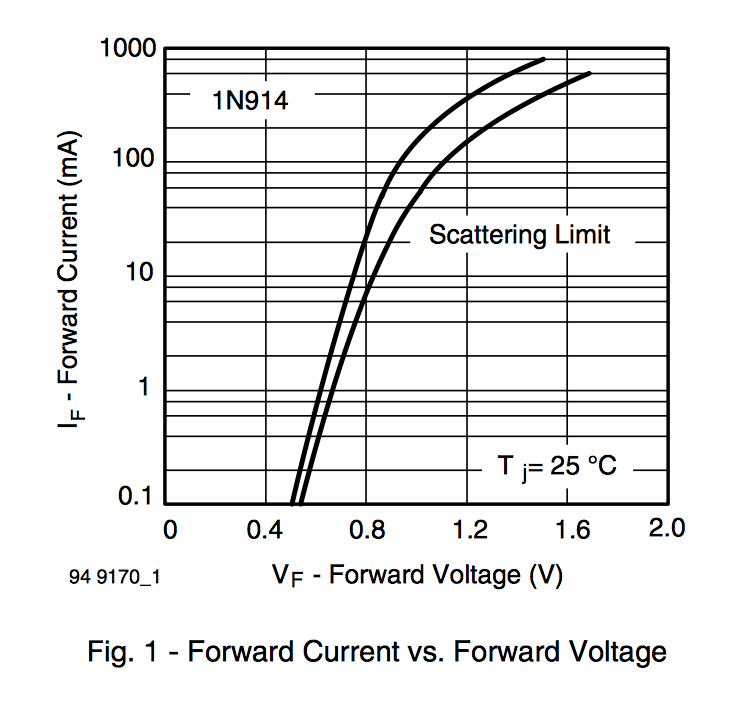
\includegraphics[height=0.25\textheight]{figs/labs/diode/1N914.png} &
\begin{picture}(200,100)
\put(0,0){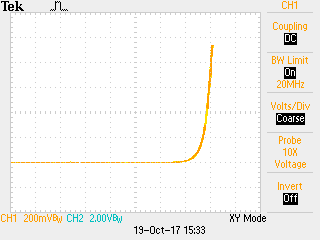
\includegraphics[height=0.25\textheight]{figs/labs/diode/diodeiv.png}}
\put(10,52){$0~mA$}
\put(10,70){$0.2~mA$}
\put(10,88){$0.4~mA$}
\put(10,106){$0.6~mA$}
\put(10,124){$0.8~mA$}
\put(10,142){$1.0~mA$}
\end{picture}\\
(a) & (b) \\
\end{tabular}
\caption{\label{fig:diodeiv} IV curves for the1N914 from (a) data sheet, and (b) as you will measure in this lab.  In the scope trace, the Channel 2 ($Y$) with scale set to $2~\rm V$ measures the voltage across a $10~\rm k\Omega$ resistor, so each division corresponds to $200~\rm \mu A$ as indicated. 
}
\end{center}
\end{figure}


\begin{measurement}
Set the scope to XY mode, and reproduce the diode IV curve in
Fig~\ref{fig:diodeiv}b. Sketch the curve in your logbook. Make sure to
include enough details so that one can read approximate values from
it. From your IV curve, estimate the voltage you expect across the
diode for a current of $1~\rm mA$. Record it in your logbook together
with an estimated uncertainty.
\end{measurement}

\begin{measurement}
The component data sheet in Fig.~\ref{fig:diodeiv}a shows the
Scattering Limit IV curves for the 1N914.  Typical 1N914 diodes will
have an IV curve that falls somewhere between the two curvers.
Estimate the voltage you expect across the diode for a current of
$1~\rm mA$ and the uncertainty, by considering the range of values consistent with the Scattering Limit.  Does your measured value agrees with this
expected value?
\end{measurement}

\section{Rectifying an AC Signal}

\begin{figure}[htbp]
\begin{center}
\begin{circuitikz}[line width=1pt, scale = 0.8, transform shape]
\draw (0,0) node[ground,yscale=2.0]{} to[sinusoidal voltage source,bipoles/length=1.5cm] ++(0,4) to[short] ++(2,0) coordinate(B);
\draw (B) to[resistor,l_=$R_1$] ++(0,-2) coordinate(A) to[diode,l_=$D_1$] ++(0,-2) coordinate(G) to[short,-*] ++(-2,0);
\draw (A) to[short,*-o] ++(0.75,0) node[right]{A};
\draw (B) to[short,*-o] ++(0.75,0) node[right]{B};
\draw (G) to[short,*-o] ++(0.75,0) node[right]{G};
\end{circuitikz} 
\caption{A diode rectification circuit.}
\label{fig:rect}
\end{center}
\end{figure}

Set your function generator to provide an AC source with frequency
$100~\rm Hz$ and peak-to-peak voltage $V_{\rm pp}=5~\rm V$.  Build the
circuit in Fig.~\ref{fig:rect} using a 1N914 diode for $D$ and
$R=1.8~\rm k\Omega$. With your scope probe ground shield clips both properly connected to
the ground at $G$, monitor the voltage at points $A$ and $B$.
\begin{measurement}  Sketch the voltage across the resistor $R$ and the voltage supplied by
the function generator versus time on the same plot in your lab book. Make sure to include enough details so that one can read approximate values from it. \end{measurement}

\begin{measurement}  Using your scopes amplitude measurement feature, measure precisely
(i.e. to within $50~\rm mV$ precision) the voltage drop across the
diode at the peak current value, by measuring the difference between
Channel 1 and Channel 2 of your scope at the peak.  Is this operating
point consistent with your results from the previous section and
the calculation above? \end{measurement}

\section{Building a DC voltage source}

Now build the DC source circuit in Fig.~\ref{fig:fwrect} using a 1N914
diode for $D_1 = D_2 = D_3 = D_4$ and $R_{\rm L}=18~\rm k\Omega$.  Adjust your function
generator to provide a peak-to-peak voltage $V_{\rm pp} = 20~\rm V$.

\begin{figure}[htbp]
\begin{center}
\begin{circuitikz}[line width=1pt, scale = 0.8, transform shape]
\draw (0,0) coordinate(G) to[sinusoidal voltage source,bipoles/length=1.5cm] ++(0,4) to[short] ++(2.0,0) to[short] ++(2.0,0); 
\draw (2,2) to[diode,l_=$D_1$,-*] ++(0,-2); 
\draw (2,2) to[diode,l=$D_2$,-*] ++(0,2); 
\draw (4,4) to[diode,l_=$D_3$] ++(0,-2); 
\draw (4,0) to[diode,l=$D_4$] ++(0,2);
\draw (0,0) to[short,*-] (4,0);
\draw (0,0) node[ground,yscale=2.0]{};
\draw (0,0) to[short,-o] ++(-0.75,0) node[left]{G};
\draw (2,1.8) to[short,*-] ++(4,0) -- ++(0,-1.8) -- ++(2,0) coordinate (Y);
\draw (4,2.2) to[short,*-] ++(2,0) -- ++(0,1.8) -- ++(2,0) coordinate (X);
\draw (X) to[short] ++(0,-1) coordinate(B) to[R,l=$R_{\rm L}$] ++(0,-2.0) coordinate(A) to[short] (Y);
\draw (A) to[short,*-o] ++(0.75,0) node[right]{A};
\draw (B) to[short,*-o] ++(0.75,0) node[right]{B};
\end{circuitikz}
\caption{A full-wave rectifier.}
\label{fig:fwrect}
\end{center}
\end{figure}

To measure the performance of our DC source, we would like to measure
the voltage across the resistor $R_L$ on the scope.  However, notice
that the ground for the circuit is located at point $G$, so you cannot
measure the voltage between $A$ and $B$ using a single probe.  To
make the measurement, connect both probe ground shield clips to the
point $G$ as required, and connect the probe tips to points $A$ and
$B$.  Next, use your scope's Math mode to subtract Channel 1 to from
Channel 2.  The result of this operation is the voltage across the
resistor $R_{\rm L}$.

\begin{measurement}
In your logbook, sketch the current as a function of time for a few
cycles, and measure the amplitude. Make sure to include enough details
that one can read approximate values from it.  Explain the shape and
the amplitude.
\end{measurement}


\section{Controlling the Ripple}

The ripple voltage (the residual AC voltage after rectification) 
for a full-wave rectifier with a capacitance $C$ is given by:
\begin{displaymath}
\Delta V = \frac{I_{\rm max}}{2 f C}
\end{displaymath}
You might notice that this differs from the equation for a half-wave
rectifier by a factor of two: $f \to 2 f$.  This is because the
full-wave rectifier uses both the positive and negative halves of the
AC signal, so the rectified AC signal has twice the frequency of the
original.

\begin{measurement} \label{meas:ripple}
Add a capacitor with $C=1~\rm{\mu F}$ to your circuit, as in Fig.~\ref{fig:fwrectc} and sketch the resulting waveform for the voltage across the load resistor as measured with your scope.  Estimate the ripple voltage.  \end{measurement}


\begin{measurement}  \label{meas:ripple2} As your DMM is a handheld device that is not DC coupled, you may use it to measure the voltage across $R_L$ directly.  Using your DMM, measure the voltage across $R_L$ in both AC and DC mode. Record those values in your log book. \end{measurement}

This is a \textbf{sign-off point} for this lab. \\

For the last tweak, you are going to use a large electrolytic
capacitor.  {\bf These capacitors are polarized, and will likely ``let
  the smoke out'' if you install them the wrong way.}  
 \begin{measurement}   Making sure the
negative terminal is connected as indicated in Fig.~\ref{fig:fwrectc},
install a $C=100~\rm \mu F$ electrolytic capacitor in your circuit and
measure the ripple voltage. Record the value in your log book. Note down your observation when comparing this value to the measurements in Meas.~\ref{meas:ripple} and ~\ref{meas:ripple2}. \end{measurement}

\begin{figure}[htbp]
\begin{center}
\begin{circuitikz}[line width=1pt, scale = 0.8, transform shape]
\draw (0,0) coordinate(G) to[sinusoidal voltage source,bipoles/length=1.5cm] ++(0,4) to[short] ++(2.0,0) to[short] ++(2.0,0); 
\draw (2,2) to[diode,l_=$D_1$,-*] ++(0,-2); 
\draw (2,2) to[diode,l=$D_2$,-*] ++(0,2); 
\draw (4,4) to[diode,l_=$D_3$] ++(0,-2); 
\draw (4,0) to[diode,l=$D_4$] ++(0,2);
\draw (0,0) to[short,*-] (4,0);
\draw (0,0) node[ground,yscale=2.0]{};
\draw (0,0) to[short,-o] ++(-0.75,0) node[left]{G};
\draw (2,1.8) to[short,*-] ++(4,0) -- ++(0,-1.8) -- ++(2,0) coordinate (Y);
\draw (4,2.2) to[short,*-] ++(2,0) -- ++(0,1.8) -- ++(2,0) coordinate (X);
\draw (Y) to[pC,l=$C$] (X);
\draw (X) to[short,*-] ++(2,0) coordinate (X);
\draw (Y) to[short,*-] ++(2,0) coordinate (Y);
\draw (X) to[short] ++(0,-1) coordinate(B) to[R,l=$R_{\rm L}$] ++(0,-2.0) coordinate(A) to[short] (Y);
\draw (A) to[short,*-o] ++(0.75,0) node[right]{A};
\draw (B) to[short,*-o] ++(0.75,0) node[right]{B};
\end{circuitikz}
\caption{A full-wave rectifier with ripple voltage limiting capacitor.  When using a polarized electrolytic capacitor, make certain that the negative terminal is connected to the lower half of the figure, as indicated. In other words, the curved sign of the symbol for a polarized electrolytic capacitor is always negative. 
}
\label{fig:fwrectc}
\end{center}
\end{figure}

 

